\begin{figure}[H]
\centering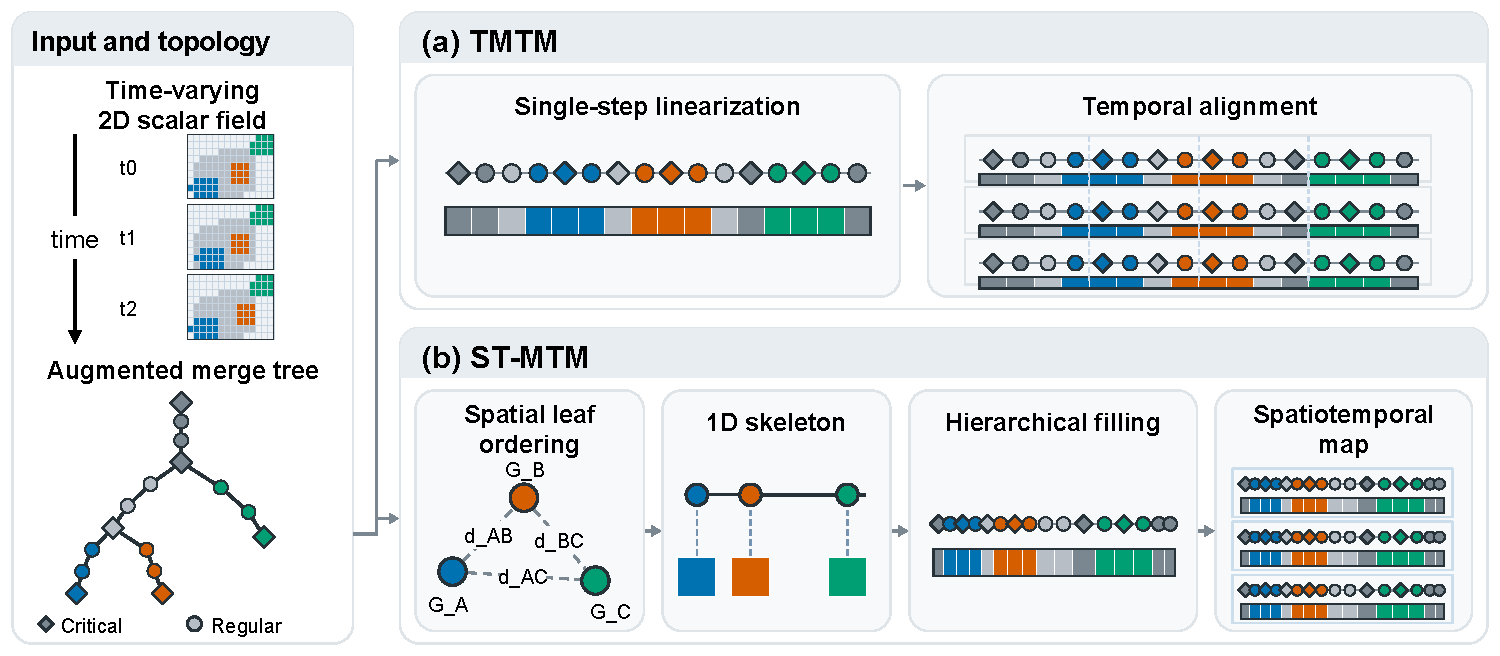
\includegraphics[width=\linewidth]{figures/Fig2.pdf}
\caption{Conceptual comparison of preceding merge-tree map workflows, redrawn and extended from ST-MTM Figs.~1 and 3~\cite{STMTM:2026}. Both use augmented trees with critical (diamond) and regular (circle) nodes. (a) TMTM~\cite{Koepp:2023:TMTM} linearizes samples within subtrees and optimizes temporal alignment. (b) ST-MTM constructs a distance-aware 1D skeleton, fills its scalar domain, and assembles the map. Branch/sample identities use the same palette throughout the schematics: $A$ (blue), $B$ (orange), and $C$ (green); internal groups are grey.}
\label{fig:prior_work}
\end{figure}
